\chapter{Introduction and Background Research}

\setlength{\parindent}{1em}
\setlength{\parskip}{0em}
\justifying

% You can cite chapters by using '\ref{chapter1}', where the label must
% match that given in the 'label' command, as on the next line.
\label{chapter1}

% Sections and sub-sections can be declared using \section and \subsection.
% There is also a \subsubsection, but consider carefully if you really need
% so many layers of section structure.
\section{Introduction}

Rendering is the process of generating images, or \textit{frames}, of a virtual world. Real-time rendering requires that the generation of these frames is done at a fast enough rate so that the viewer feels they are taking part in an immersive, dynamic experience. Typically, this rate needs to be at least 30 FPS (Frames Per Second), with 60 FPS and beyond being desirable \cite{EffectsOfFrameRate}. This imposes a maximum time budget of 33 to 16 milliseconds in which each frame must be generated, the \textit{frame time}. Real-time rendering presents a compelling problem: how can the visual fidelity of a rendered scene be maximised, whilst adhering to this strict computational budget.

Rendering can be performed using one of two techniques, ray tracing or rasterization. Ray tracing is based on a model that is analogous to how humans perceive light and colour in the real-world. In the real-world, rays of light are produced from many sources, bounce from one object to the next, and eventually reach the viewers eyes. Ray tracing models this same process, but in reverse, with the rays originating from the views eyes, and being traced back to their sources. Provided enough rays are sampled, this approach produces very realistic images. Although ray tracing is the standard in the realm of movie production, its expensive computational requirements lead to frame times in the region of minutes instead of milliseconds~\cite{PixarCars}. Aside from so notable exceptions\footnote{With the introduction of hardware accelerated ray tracing on consumer GPUs~\cite{NvidiaTuringArchitecture}, the use of ray tracing to render specific visual phenomena, such as reflections, has seen use in some modern games~\cite{Battlefield5RayTracing}.}, this prohibits its use in real-time applications. As a result, real-time rendering employs another technique, rasterization.

With rasterization, each object in the world is composed of an arrangement of primitive shapes, most commonly, triangles, and their material is described through a number of parameters. When rendering, the world is transformed and projected onto a 2D plane. Within this plane, a fixed region maps to the space of the output image; all triangles that lie outside this region are clipped. The remaining triangles are then split into granular pieces, called \textit{fragments}. A colour is calculated for each fragment by evaluating the amount of light that shines on that fragment in the world, and then how that light interacts with the material of the object that fragment belongs to. Performing this calculation is called \textit{shading}, and how it is done is defined by a \textit{shading model}. After resolving which fragments lie on top of which others, the final image is presented to the user. This whole rasterization process is referred to as the graphics rendering pipeline, and dedicated hardware has been developed to carry it out, the \textit{Graphics Processing Unit} (GPU).

The appearance of the final rendered frames is largely determined by the shading model, and therefore the choice of such a model is crucial. For a long time, the standard shading model used for photo-realistic real-time rendering was Blinn-Phong; it was utilised in popular game engines, and was the default model used in OpenGL's fixed function pipeline~\cite{UnityBlinnPhong}~\cite{UnrealBlinnPhong}~\cite{OpenGLBlinnPhongFixedFunction}. Blinn-Phong is an empirical model: it is based on human observations of how light interacts with materials, rather than the underlying real-world physical rules that govern those interactions~\cite{PhongShading}. Blinn-Phong can produce reasonably realistic images, and is computationally inexpensive - a very desirable trait for real-time rendering. However, due to its non-physically based nature, Blinn-Phong has many issues. Paramount amongst which is its inability to render certain physical phenomena, which limits the realism of rendered frames. Furthermore, the parameters of Blinn-Phong that are used to specify material properties, bear little relation to the characteristics of physical materials. This problem manifests itself in a tight coupling between material parameters and lighting conditions. In order to accurately depict the same physical material under different lighting conditions, it may be necessary to specify differing values for these parameters. This reduces the reusability of assets, making artist workflow more difficult.

In an effort to alleviate these issues, the replacement of Blinn-Phong in favour of physically based shading models has seen widespread adoption. Such models work by evaluating equations that simulate the real world physical interaction of light and objects. Using these models for shading is known as \textit{Physically Based Shading} (PBS), and their use in the wider rendering pipeline is called \textit{Physically Based Rendering} (PBR). PBS represented a seismic shift in the real-time rendering industry, with major game engines migrating to a PBR pipeline~\cite{RealShadingInUnreal}~\cite{movingFrostbitetoPBR}.

The aim of this project is to investigate the use of physically based shading models in real time rendering. Specifically, I will seek to highlight the benefits of PBS when compared to the technology is superseded, Blinn-Phong shading.

The advantages of using PBS over Blinn-Phong shading can be broadly categorised into two groups: the improvements to artist workflow; and the improved photorealism. As mentioned previously, because of how materials are defined in Blinn-Phong shading they are often not portable between different lighting environments. In contrast, the parameters that determine materials in PBS are based on physical properties. This permits the reuse of materials and assets over different lighting configurations~\cite{movingFrostbitetoPBR}~\cite{SIGGRAPH2020Course}. Burley outlines how this reduction in the need for "material 're-do's" yields an extremely significant improvement to artist workflow~\cite{Burley2012Physically}. Although these benefits are an important motivating factor for using PBS, the practical issues that arise from trying to investigate and quantify them (I don’t have access to a team of artists) mean that this report will focus solely on exploring those advantages in the latter category – how does PBS render frames that are more photorealistic than Blinn-Phong?

Answering this question by simply commenting on the general perceived realism of a frame when compared to another, is a largely subjective exercise. Instead, in a concerted effort to be as objective as possible, I will examine the benefits of PBS by identifying physical phenomena that it models in its rendered frames, but that are absent when using Blinn-Phong shading. To this end, I will be developing a piece of software that can render scenes using both Blinn-Phong shading, and PBS.

\section{Mathematical Notation}

When reasoning about different mathematical expressions and models, it's of vital importance that a standard, coherent notation is used throughout.

\begin{center}
	\begin{tabular}{ c c }
		\hline
		\begin{math}\vect{n}\end{math} & Normal vector \\
		\begin{math}\vect{l}\end{math} & Light direction \\
		\begin{math}\vect{v}\end{math} & View vector \\
		\begin{math}\vect{c}_{x}\end{math} & The RGB triplet vector representing the colour of \begin{math}x\end{math}\\
		\begin{math}\vect{a}\cdot\vect{b}\end{math} & The dot product of vectors \begin{math}\vect{a}\end{math} and \begin{math}\vect{b}\end{math} \\
		\begin{math}\norm{\vect{a}}\end{math} & The norm of vector \begin{math}\vect{a}\end{math} \\
		\begin{math}x^+\end{math} & Clamp \begin{math}x\end{math} to \begin{math}0\end{math} if \begin{math}x<0\end{math} \\
		\hline
	\end{tabular}
\end{center}

% Must provide evidence of a literature review. Use sections
% and subsections as they make sense for your project.
\section{Literature review}

The review begins with a brief discussion of the Blinn-Phong shading model; this provides the necessary background knowledge for the later comparison with physically based shading models to be performed. We then delve into the physics of how light interacts with matter, and how this pertains to shading. An exploration of the theory underpinning physically based shading models follows, and then we present several such models. After, we consider how lights can be represented in a physical manner. Finally, we finish by focusing on the wider PBR aspect with a discussion on how we store pixel colours, and the transformations that need to be applied before passing those colours to the display.

\subsection{Blinn-Phong Shading}

\subsubsection{Phong Model}

In 1975, Phong introduced a simple shading model for rendering realistic images~\cite{PhongShading}. The original model is parametrised as the sum of two terms, \textit{diffuse} and \textit{specular}, but in practice it is commonly supplemented with a third term, \textit{ambient}. Each one describes the contribution of a different lighting component. Splitting shading into the evaluation of a diffuse and specular term is common practice, and the physical basis for doing this is explained in section \ref{PhysicsOfLightMatterInteraction}.

An ideal diffuse surface follows Lambert's law: light incident onto a point will be diffused in all directions equally~\cite{Lambert}. Therefore, the determining factor in the appearance of such surfaces is the intensity of the incident light, which is a function of the direction of incident light and the orientation of the shaded surface. The diffuse term encodes the lighting effects of parity between a primitive's surface orientation and the direction of the light, with surfaces facing the light being illuminated more intensely than those facing away from it. This behaviour is formulated as:

\begin{center}
	\begin{math}\vect{c}_{shaded_{diff}} = \vect{c}_{surface_{diff}}\vect{c}_{light_{diff}}(\vect{n}\cdot\vect{l})^+\end{math}
\end{center}

\begin{math}\vect{c}_{shaded_{diff}}\end{math}, \begin{math}\vect{c}_{surface_{diff}}\end{math}, and \begin{math}\vect{c}_{light_{diff}}\end{math} are the RGB triplets that represent the diffuse colour of the shaded fragment, the diffuse colour of the surface, and the diffuse colour of the incident light respectively. This separation of the light and surface colours into separate components was not present in Phong's original model. However, many implementations have increased the flexibility of the model by exposing these additional parameters~\cite{LightingModelForComputerAnimators}. The \textit{normal}, \begin{math}\vect{n}\end{math}, is the unit vector pointing away from the surface at the shaded point, giving the orientation of the surface.  The \textit{light direction}, \begin{math}\vect{v}\end{math}, is the unit vector pointing in the direction of the incident light. See Figure \ref{fig:PrincipleVectors} for an illustration of the principle vectors used in the Phong shading model (and indeed, by most shading models). The dot product of two unit vectors is equivalent to taking the cosine of the angle between them. Therefore, \begin{math}(\vect{n}\cdot\vect{l})^+\end{math} will increase from 0 to 1 as the angle between the incident light direction and the surface normal decreases. Thus, the more aligned the surface orientation and light direction are, the greater the intensity of the diffuse term. Negative values of the dot product indicate that the light direction is underneath the surface. In these cases the light is not incident upon the surface at all, so the dot product is clamped to 0.

The specular term of the model captures the ability for surfaces to exhibit highlights due to surface reflections. When light is incident upon a surface, it will experience some reflection, and when the reflected light is aligned with the direction of the viewer, this is perceived as a region of increased illumination, a \textit{specular highlight}. The formula for the specular term is:

\begin{center}
	\begin{math}\vect{c}_{shaded_{spec}} = \vect{c}_{surface_{spec}}\vect{c}_{light_{spec}}((\vect{r}\cdot\vect{v})^+)^{surface_{shininess}}\end{math} \\
\end{center}

Where \begin{math}\vect{r}\end{math} is the reflection of the incident light about the surface normal, and is defined as:

\begin{center}
	\begin{math}\vect{r} = 2(\vect{n}\cdot\vect{l})\vect{n} - \vect{l}\end{math}	
\end{center}

The RGB triplets are similar to those in the diffuse equation, except these are specific to the specular response. Phong's original model had the colour of the specular highlight be the same as the overall colour of the light (not split into separate diffuse and specular components). This gave all materials an overly plastic appearance. Introducing the \begin{math}\vect{c}_{surface_{spec}}\end{math} and \begin{math}\vect{c}_{light_{spec}}\end{math} variables allows for the colour of the specular highlight to be fully configurable, mitigating this issue~\cite{LightingModelForComputerAnimators}. The \textit{view vector}, \begin{math}\vect{v}\end{math}, is the unit vector pointing in the direction of the viewer. The dot product measures the alignment between the view direction, and the direction of the reflected incident light. The \begin{math}surface_{shininess}\end{math} parameter determines the concentration of the reflected light rays. The higher the value, the more focused the reflected rays are, the smaller the specular highlight becomes, and the shinier the object appears. Typical values range from 1 to 100.

Finally, we have the ambient term. In the model developed so far, if a shaded point is not directly visible from a light source, then it will be black. In reality, such points are never completely unilluminated - rays from light sources will bounce around the environment, eventually lighting these obscured areas. So far we have only considered \textit{direct lighting}; the ambient term is used to crudely approximate the illumination that is a consequence of this \textit{indirect lighting}:

\begin{center}
	\begin{math}\vect{c}_{shaded_{ambi}} = \vect{c}_{surface_{ambi}}x\end{math}
\end{center}

\begin{math}\vect{c}_{surface_{ambi}}\end{math} controls the colour of the ambient shading. Typically, it is just set equal to \begin{math}\vect{c}_{surface_{diff}}\end{math}. \begin{math}x\end{math} is a constant value defined for the whole scene, rather than per light, and controls the amount of indirect lighting that occurs. A value of \begin{math}x = 0.2\end{math} is commonly used.

These three terms are summed together to give the overall Phong shading model:

\begin{center}
	\begin{math}\vect{c}_{shaded} = \vect{c}_{shaded_{ambi}} + \vect{c}_{shaded_{diff}} + \vect{c}_{shaded_{spec}}\end{math}
\end{center}

\begin{figure}[h]
	\centering
	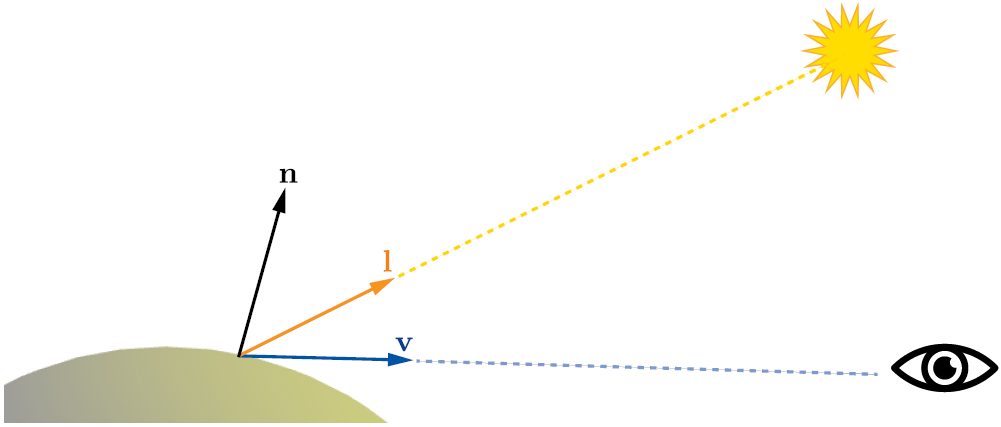
\includegraphics[width=8cm]{PrincipleVectors}
	\caption{The surface normal \begin{math}\vect{n}\end{math}, light direction \begin{math}\vect{l}\end{math}, and view vector \begin{math}\vect{v}\end{math}~\cite{RTR4}}
	\label{fig:PrincipleVectors}
\end{figure}

\subsubsection{Blinn-Phong Model}

One of the issues with the Phong shading model is made apparent when viewing a rough (low \begin{math}shininess\end{math} value) surface from a direction close to the incident light. The corresponding reflected light vector makes an angle with the view direction that is greater than 90$^{\circ}$. In this instance, the dot product \begin{math}\vect{r}\cdot\vect{v}\end{math} evaluates to a negative value, and is thus clamped to 0, leading to no specular contribution. However, for very rough surfaces, the specular highlight is so wide that even at these greater angles, there should still be a specular contribution. See Figure \ref{fig:PhongIssue} for an illustration of the problem.

In 1977, Blinn remedied this issue by modifying the Phong shading model with a more accurate specular term~\cite{BlinnModelsOfLightReflection}. He utilised the half vector, \begin{math}\vect{h}\end{math}, dispensing with the reflected light vector, \begin{math}\vect{r}\end{math}, and replaced the existing specular dot product with \begin{math}\vect{h}\cdot\vect{n}\end{math}. \begin{math}\vect{h}\end{math} is a unit vector pointing in the direction that is halfway between the \begin{math}\vect{l}\end{math} and \begin{math}\vect{v}\end{math} vectors. It is calculated as:

\begin{center}
	\begin{math}\vect{h} = \frac{\vect{l} + \vect{v}}{\norm{\vect{l} + \vect{v}}}\end{math}
\end{center}

Blinn's specular term emulates the overall behaviour of the original Phong term. As the (now conceptual) reflection vector \begin{math}\vect{r}\end{math} aligns with \begin{math}\vect{v}\end{math}, so does the half vector \begin{math}\vect{h}\end{math} align with the surface normal \begin{math}\vect{n}\end{math}. Crucially though, \begin{math}\vect{h}\cdot\vect{n}\end{math} will only evaluate to a negative value, and subsequently be clamped to 0, if \begin{math}\vect{l}\end{math} or \begin{math}\vect{v}\end{math} is beneath the surface. Therefore, the scenario in which rough surfaces were being shaded incorrectly with no specular contribution, is resolved. See \ref{fig:BlinnFix} for an illustration.

\begin{figure}[h]
	\begin{subfigure}{0.48\textwidth}
		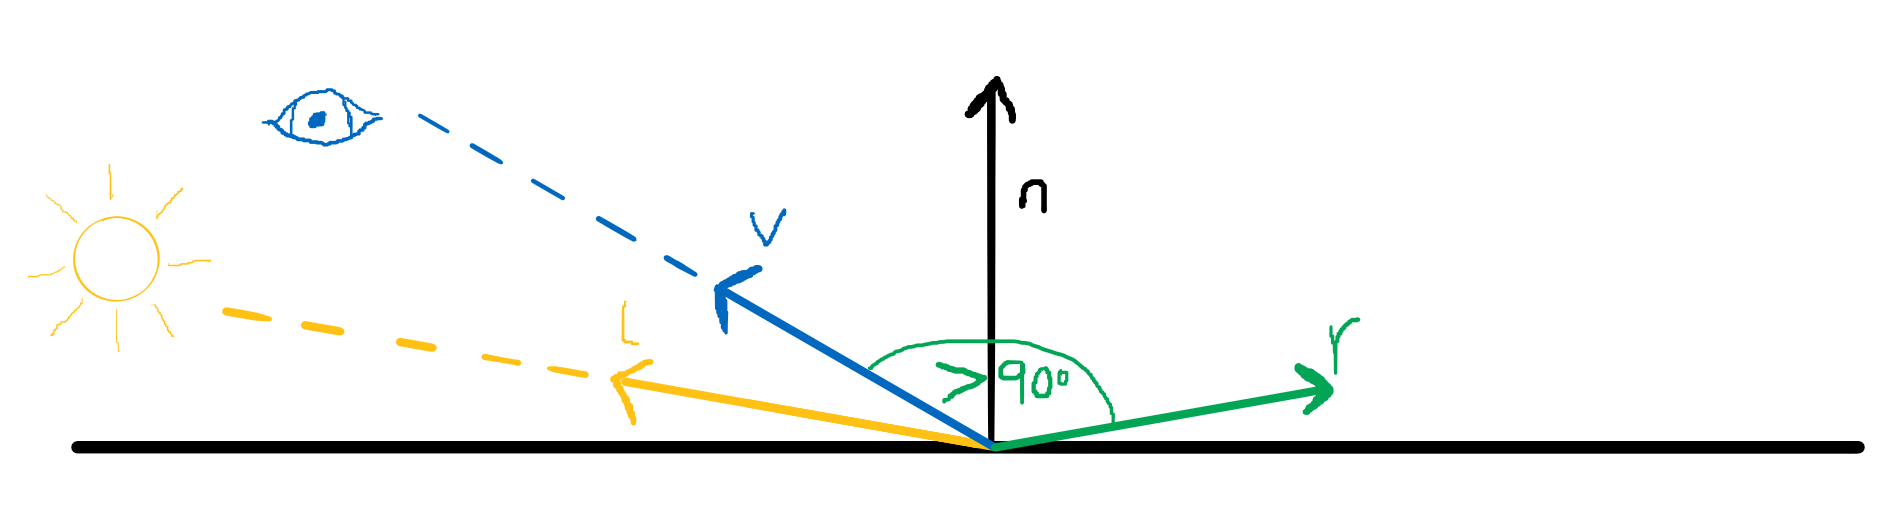
\includegraphics[width=\linewidth]{PhongIssue}
		\caption{The angle between \begin{math}\vect{r}\end{math} and \begin{math}\vect{v}\end{math} can exceed 90$^{\circ}$ whilst \begin{math}\vect{l}\end{math} and \begin{math}\vect{v}\end{math} are still above the surface}
		\label{fig:PhongIssue}
	\end{subfigure}
	\hspace*{\fill}
	\begin{subfigure}{0.48\textwidth}
		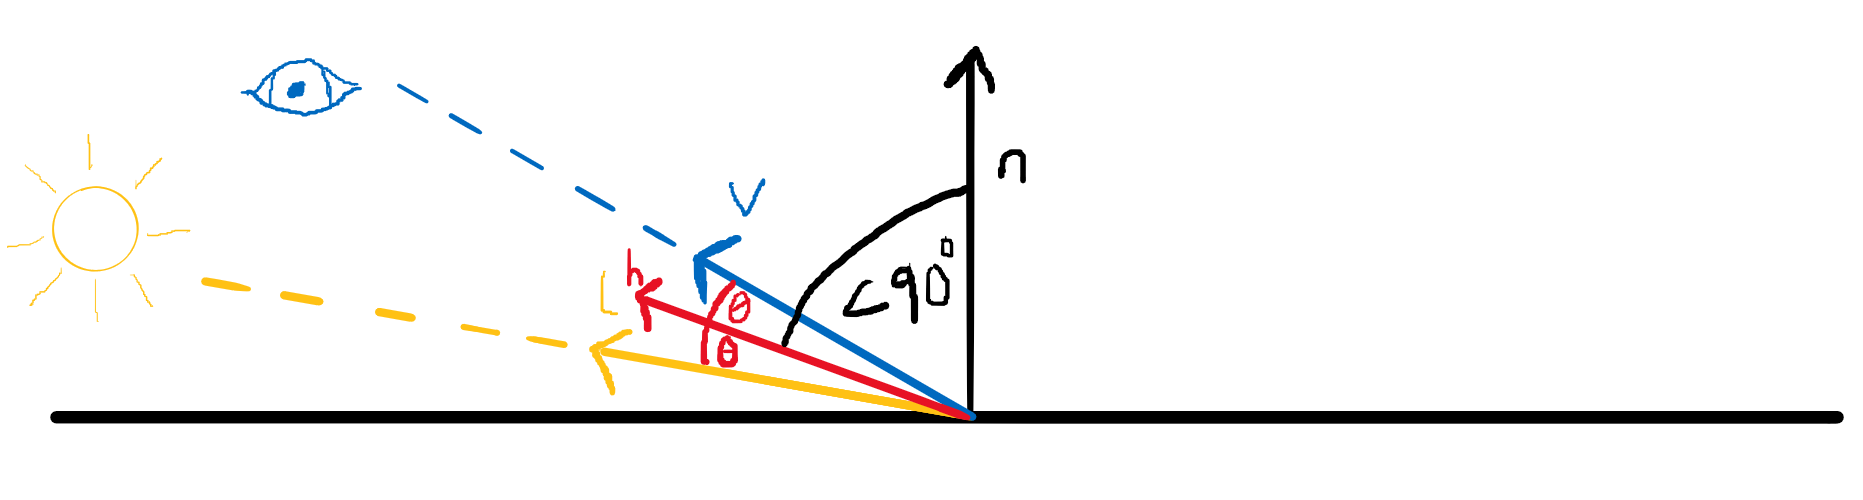
\includegraphics[width=\linewidth]{BlinnFix}
		\caption{The angle between \begin{math}\vect{h}\end{math} and \begin{math}\vect{n}\end{math} can't exceed 90$^{\circ}$ without \begin{math}\vect{l}\end{math} and \begin{math}\vect{v}\end{math} being below the surface }
		\label{fig:BlinnFix}
	\end{subfigure}
	\caption{}
\end{figure}

Blinn's modification to the Phong model is known as the Blinn-Phong shading model, and it produces more realistic images than the original. The model is formulated as:

\begin{center}
	\begin{math}\vect{c}_{shaded} = p_{ambi} + p_{diff}(\vect{n}\cdot\vect{l})^+ + p_{spec}((\vect{h}\cdot\vect{n})^+)^{surface_{shininess}}\end{math}
\end{center}

where

\begin{center}
	\begin{math}p_{ambi} = \vect{c}_{surface_{ambi}}x\end{math} \\
	\begin{math}p_{diff} = \vect{c}_{surface_{diff}}\vect{c}_{light_{diff}}\end{math} \\
	\begin{math}p_{spec} = \vect{c}_{surface_{spec}}\vect{c}_{light_{spec}}\end{math}
\end{center}

Expressing the model in this way draws attention to the relative proportions of each component that contributes to the overall shading. These proportions, \begin{math}p\end{math}, are modulated via lighting parameters:  \begin{math}light\end{math} variables and \begin{math}x\end{math}; and material parameters: \begin{math}surface\end{math} variables.

\subsection{Physics of Light-Matter Interaction} \label{PhysicsOfLightMatterInteraction}

\begin{itemize}
	\item Physics of light?
	\item Reflectance equation
	\item BRDFs
	\begin{itemize}
		\item What makes a good BRDF (energy conservation and the reihtsz... reciprocity)
		\item Fresnel Reflectance
		\item Microfacet theory
		\item Surface reflection
		\item Subsurface reflection
	\end{itemize}
	\item Lights
	\item HDR, tonemapping and gamma correction (display encoding)
\end{itemize}

